\documentclass[12pt]{article}
\usepackage{graphicx}
\usepackage{amsmath}
\usepackage{mathtools}
\usepackage{gensymb}

\newcommand{\mydet}[1]{\ensuremath{\begin{vmatrix}#1\end{vmatrix}}}
\providecommand{\brak}[1]{\ensuremath{\left(#1\right)}}
\providecommand{\norm}[1]{\left\lVert#1\right\rVert}
\newcommand{\solution}{\noindent \textbf{Solution: }}
\newcommand{\myvec}[1]{\ensuremath{\begin{pmatrix}#1\end{pmatrix}}}
\let\vec\mathbf

\begin{document}
\begin{center}
\textbf\large{CLASS-9\\CHAPTER-10 \\ CIRCLES}

\end{center}
\section*{Excercise 10.5}

Q1. In Figure 1. A,B,C are the three points with centre O such that $\angle$BOC=30$^\circ$ and $\angle$AOB=60$^\circ$.If D is a point on the circle other than the arc ABC, find $\angle$ADC
\section*{\large Solution}
\begin{figure}[h!]
\centering
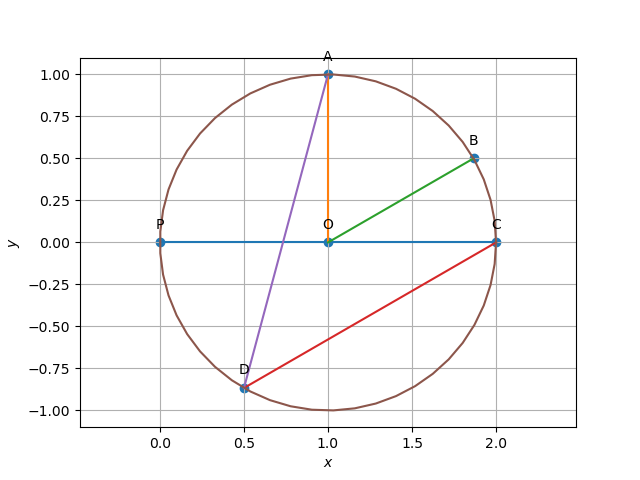
\includegraphics[width=\columnwidth]{figs/circle2.png}
\caption{}
\end{figure}
\section*{\large Construction}



The input parameters are the lengths



\begin{table}[htbp]
 \begin{center}
    \begin{tabular}{|l|c|c|c|c|c|c} \hline \textbf{Symbol}
  & \textbf{value} & \textbf{Description} \\
 \hline
O & & centre \\ \hline
$\angle$BOC &30$^\circ$ & Angle between vectors B and C  \\ \hline
$\angle$AOB&60$^\circ$&Angle between vectors A and B\\
	\hline
	$\angle$ADC&??&Angle between vectors A and C \\
	\hline
\end{tabular}   
\end{center}
\caption{\label{table:dummytable} }
\end{table}

\section*{\large Assumptions}
\begin{enumerate}
\item Let P be a point on the circle such that by expandig OC upto P we get diameter POC.
\item To find $\angle$ADC let the circle be unit circle and diameter POC on x axis.
\item Take three points C,A,D  and $\alpha$,$\beta$,$\gamma$ be three angles made by the points C,A,D with respect to diameter POC.
\end{enumerate}
From the Figure 2:
\begin{align}
\vec{\alpha} = \vec{\angle POC}= 180^\circ, 
\vec{\beta} = \vec{\angle POA} = 90^\circ,
\vec{\gamma} = \vec{\angle POD}
\end{align}
\section*{Proof:}
From assumptions the vector points C,A,D be
\begin{align}
	\vec{C} = \myvec{cos\alpha\\sin\alpha},
	\vec{A} = \myvec{cos\beta\\sin\beta},
	\vec{D} = \myvec{cos\gamma\\sin\gamma}
\end{align}
Let AC be the chord that subtends angles at the center O and at point D. The cosine of the angle subtended at point D is given by
\begin{align}
	cos(\angle ADC) = \frac{(A-D)^T(C-D)}{\norm{A-D}\norm{C-D}}
	\label{pf2-eq-3}
\end{align}
Where
 \begin{align}
	\vec{A-D} = \myvec{cos\beta - cos\gamma\\sin\beta - sin\gamma},
	\vec{C-D} = \myvec{cos\alpha - cos\gamma\\sin\alpha - sin\gamma}\\
	(A-D)^T(C-D)=\myvec{cos\beta - cos\gamma  sin\beta - sin\gamma}\\
	\label{pf2-eq-6}
	= 4\sin\frac{\alpha-\gamma}2\sin\frac{\beta-\gamma}2\cos\frac{\alpha-\beta}2\\
	\norm{A-D}^2\norm{C-D}^2 = ((\cos\alpha-\cos\gamma)^2+(\sin\alpha-\sin\gamma)^2)\\
	= 16 \sin^2\frac{\alpha-\gamma}2\sin^2\frac{\beta-\gamma}2\\
	\norm{A-D}\norm{C-D} = 4 \sin\frac{\alpha-\gamma}2\sin\frac{\beta-\gamma}2
	\label{pf2-eq-9}
\end{align}
Substituting (\ref{pf2-eq-6}) and (\ref{pf2-eq-9}) in (\ref{pf2-eq-3}),
\begin{align}
	cos(\angle ADC) &= \frac{4sin\frac{\alpha-\gamma}{2}sin\frac{\beta-\gamma}{2}cos\frac{\alpha-\beta}{2}}{4 \sin\frac{\alpha-\gamma}2\sin\frac{\beta-\gamma}2}\\
	cos(\angle ADC) &= cos\frac{\alpha-\beta}{2}
	\label{pf2-eq-11}
\end{align}
By substituting $\alpha$ and $\beta$ values in (\ref{pf2-eq-11})
\begin{align}
\angle ADC = \frac{\alpha-\beta}{2}=\frac{(180^\circ - 90^\circ )}{2}=45^\circ
\end{align}



\end{document}
